\documentclass[aspectratio=169]{beamer}
\usepackage[utf8]{inputenc}
\usepackage{graphicx} % Required for including images
\usepackage{tabularx} % For better tables

% You can uncomment a theme if you like
%\usetheme{Madrid}
%\usetheme{Boadilla}
%\usetheme{Singapore}

\title{FoldFusion-PoC: Results from a Ligand Transplantation \& Optimization Pipeline}
\author{Marius Rueve}
\date{July 21, 2025}
\institute{University of Hamburg}

\begin{document}

\begin{frame}
    \titlepage
\end{frame}

%---------------------------------------------------------------
\begin{frame}{The FoldFusion Pipeline}
    A modular, pocket-centric workflow:
    \begin{enumerate}
        \item \textbf{Pocket Prediction (DogSite3):} Identify potential binding sites on the target AlphaFold model.
        \item \textbf{Homolog Ensemble (SIENA):} Find experimentally solved structures with similar binding pockets.
        \item \textbf{Ligand Extraction:} Extract the bound ligands from these homologous structures.
        \item \textbf{Transplant \& Optimization (JAMDA):} Place the ligand into the AlphaFold model and use the JAMDA scorer to optimize its position and score the fit.
    \end{enumerate}
\end{frame}

%---------------------------------------------------------------
\section{Methods \& Evaluation Metrics}

\begin{frame}{Key Quality Metrics}
    How do we measure the quality of a transplanted ligand?
    \begin{itemize}
        \item \textbf{Local RMSD (\AA):} The Root-Mean-Square Deviation of the ligand and surrounding protein atoms compared to the original experimental structure. A \textbf{lower} value means the local binding site geometry is more accurate.
              \vspace{1em}
        \item \textbf{Transplant Clash Score (TCS):} A measure of steric clashes (atomic overlaps) between the ligand and the protein. It is calculated as $\sqrt{\sum (\text{overlap})^2 / N}$. A \textbf{lower} value means fewer clashes and a better physical fit.
    \end{itemize}
    \vfill
    \textbf{The goal of optimization is to decrease both Local RMSD and TCS.}
\end{frame}

%---------------------------------------------------------------
\section{Results}

\begin{frame}{Optimization Regarding Fit and Clashes}
    \begin{figure}
        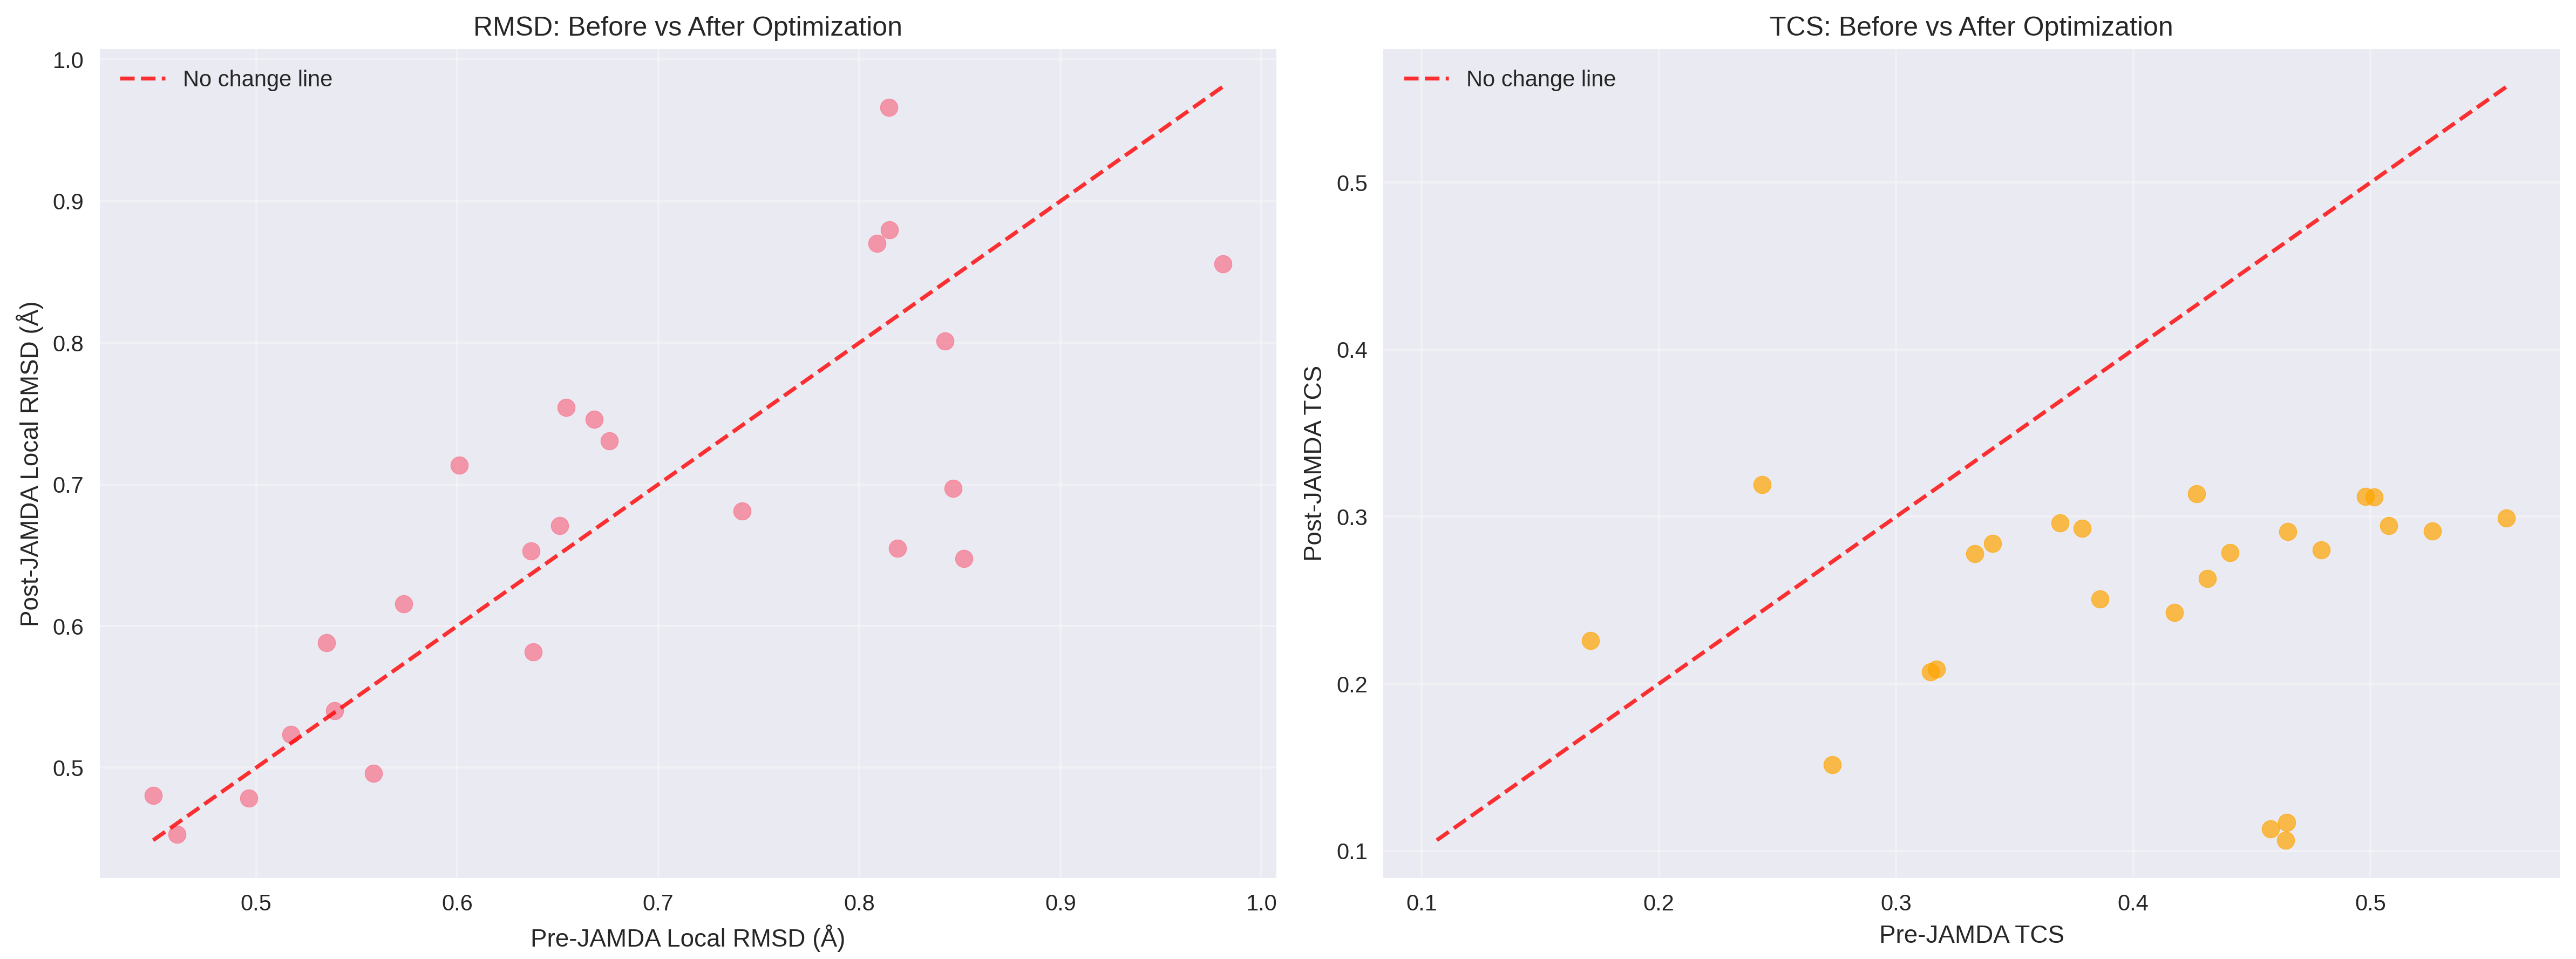
\includegraphics[width=\textwidth, keepaspectratio]{images/optimization_effectiveness_1.png}
    \end{figure}
\end{frame}
\begin{frame}{Optimization Regarding Fit and Clashes}
	\begin{figure}
		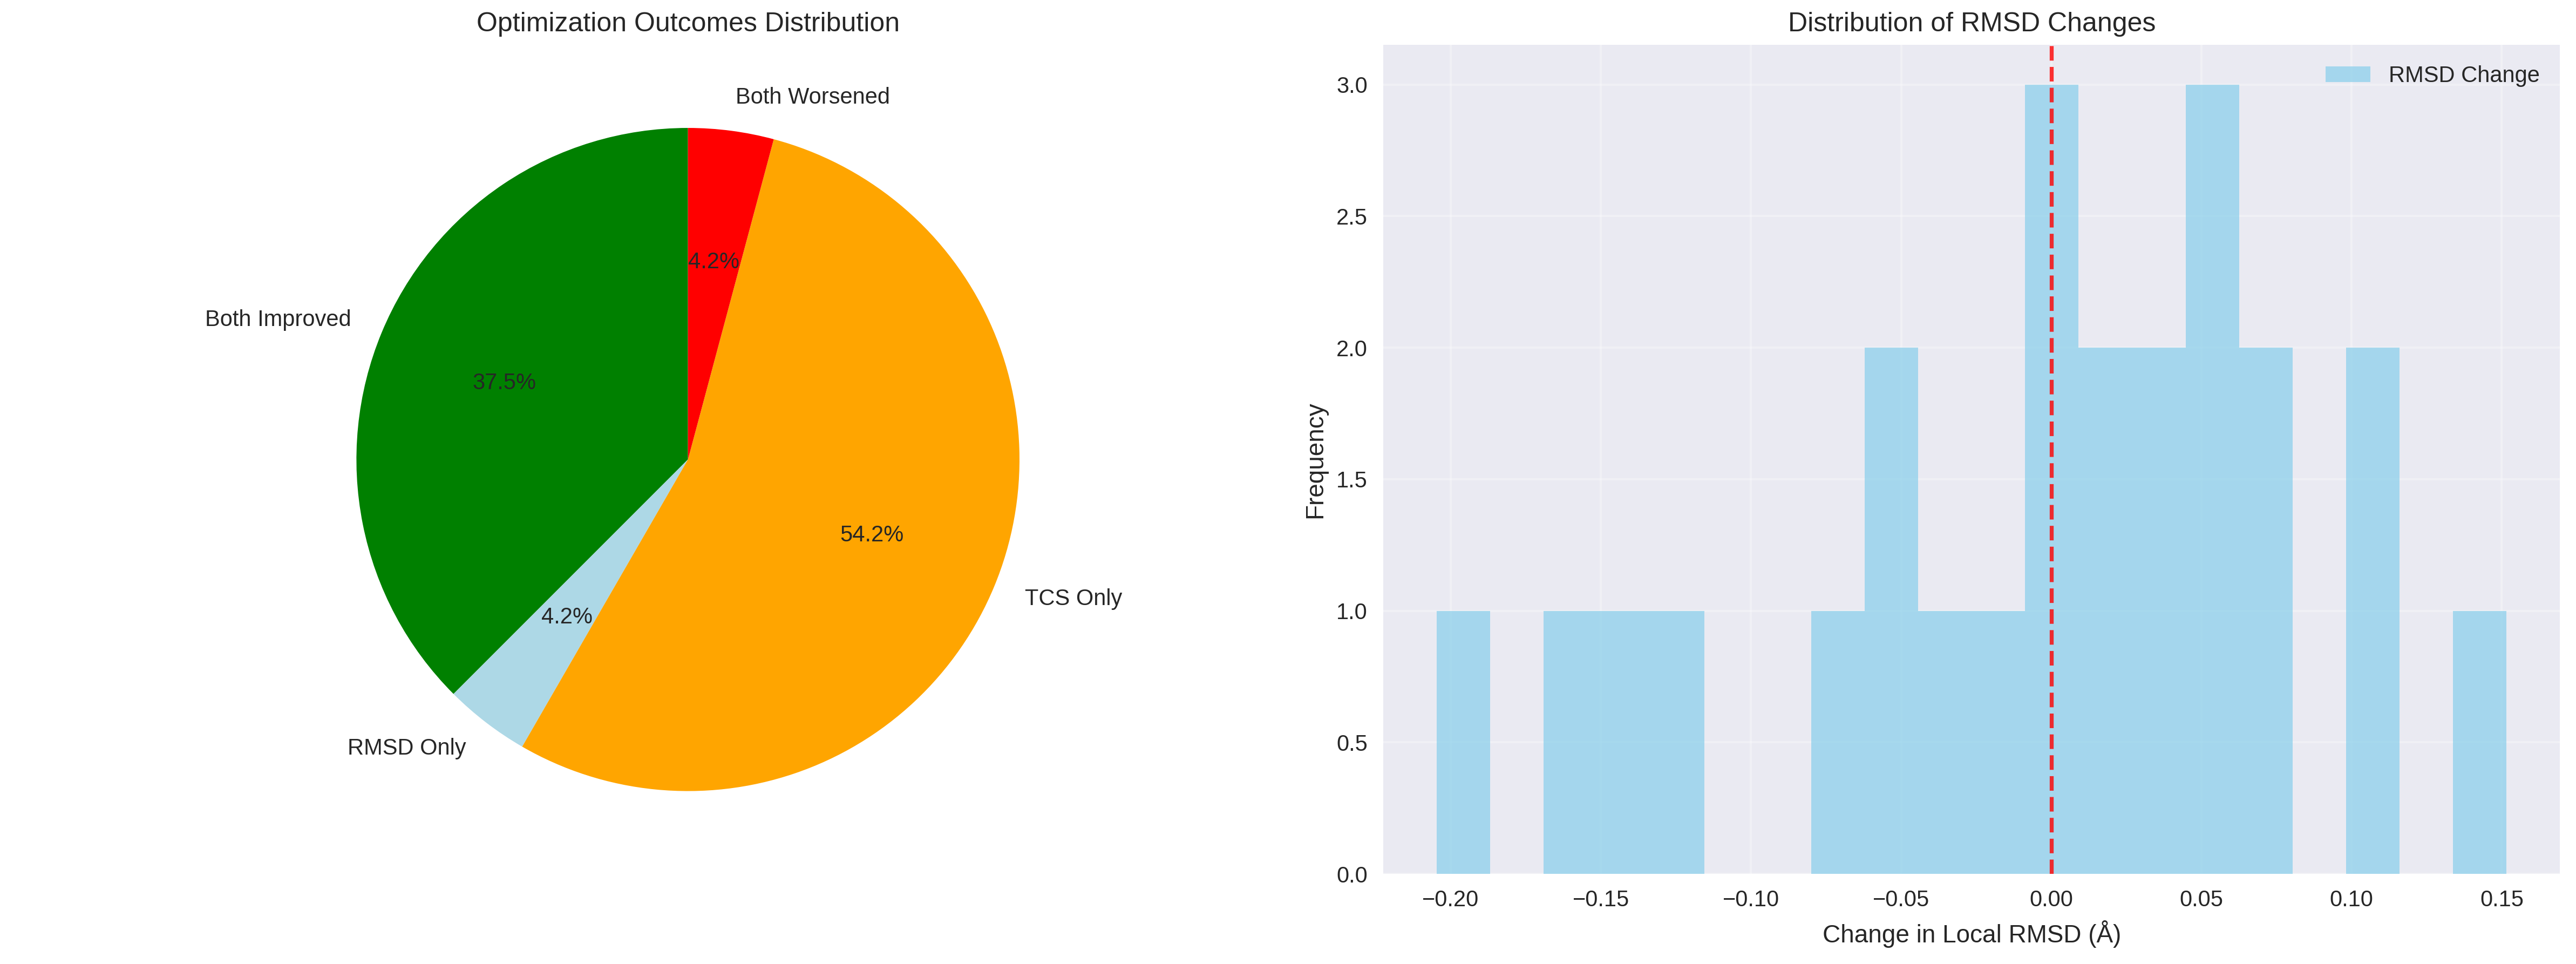
\includegraphics[width=\textwidth, keepaspectratio]{images/optimization_effectiveness_2.png}
	\end{figure}
\end{frame}
\begin{frame}{Optimization Regarding Fit and Clashes}
    \begin{itemize}
        \item The JAMDA optimization step is highly effective.
        \item \textbf{95.8\%} of transplants improved in at least one metric (Pie Chart).
        \item Both Local RMSD (geometry) and TCS (clashes) show clear improvement on average.
    \end{itemize}
\end{frame}

%---------------------------------------------------------------
\begin{frame}{Consistent Improvements Across Diverse Transplants}
    \begin{figure}
        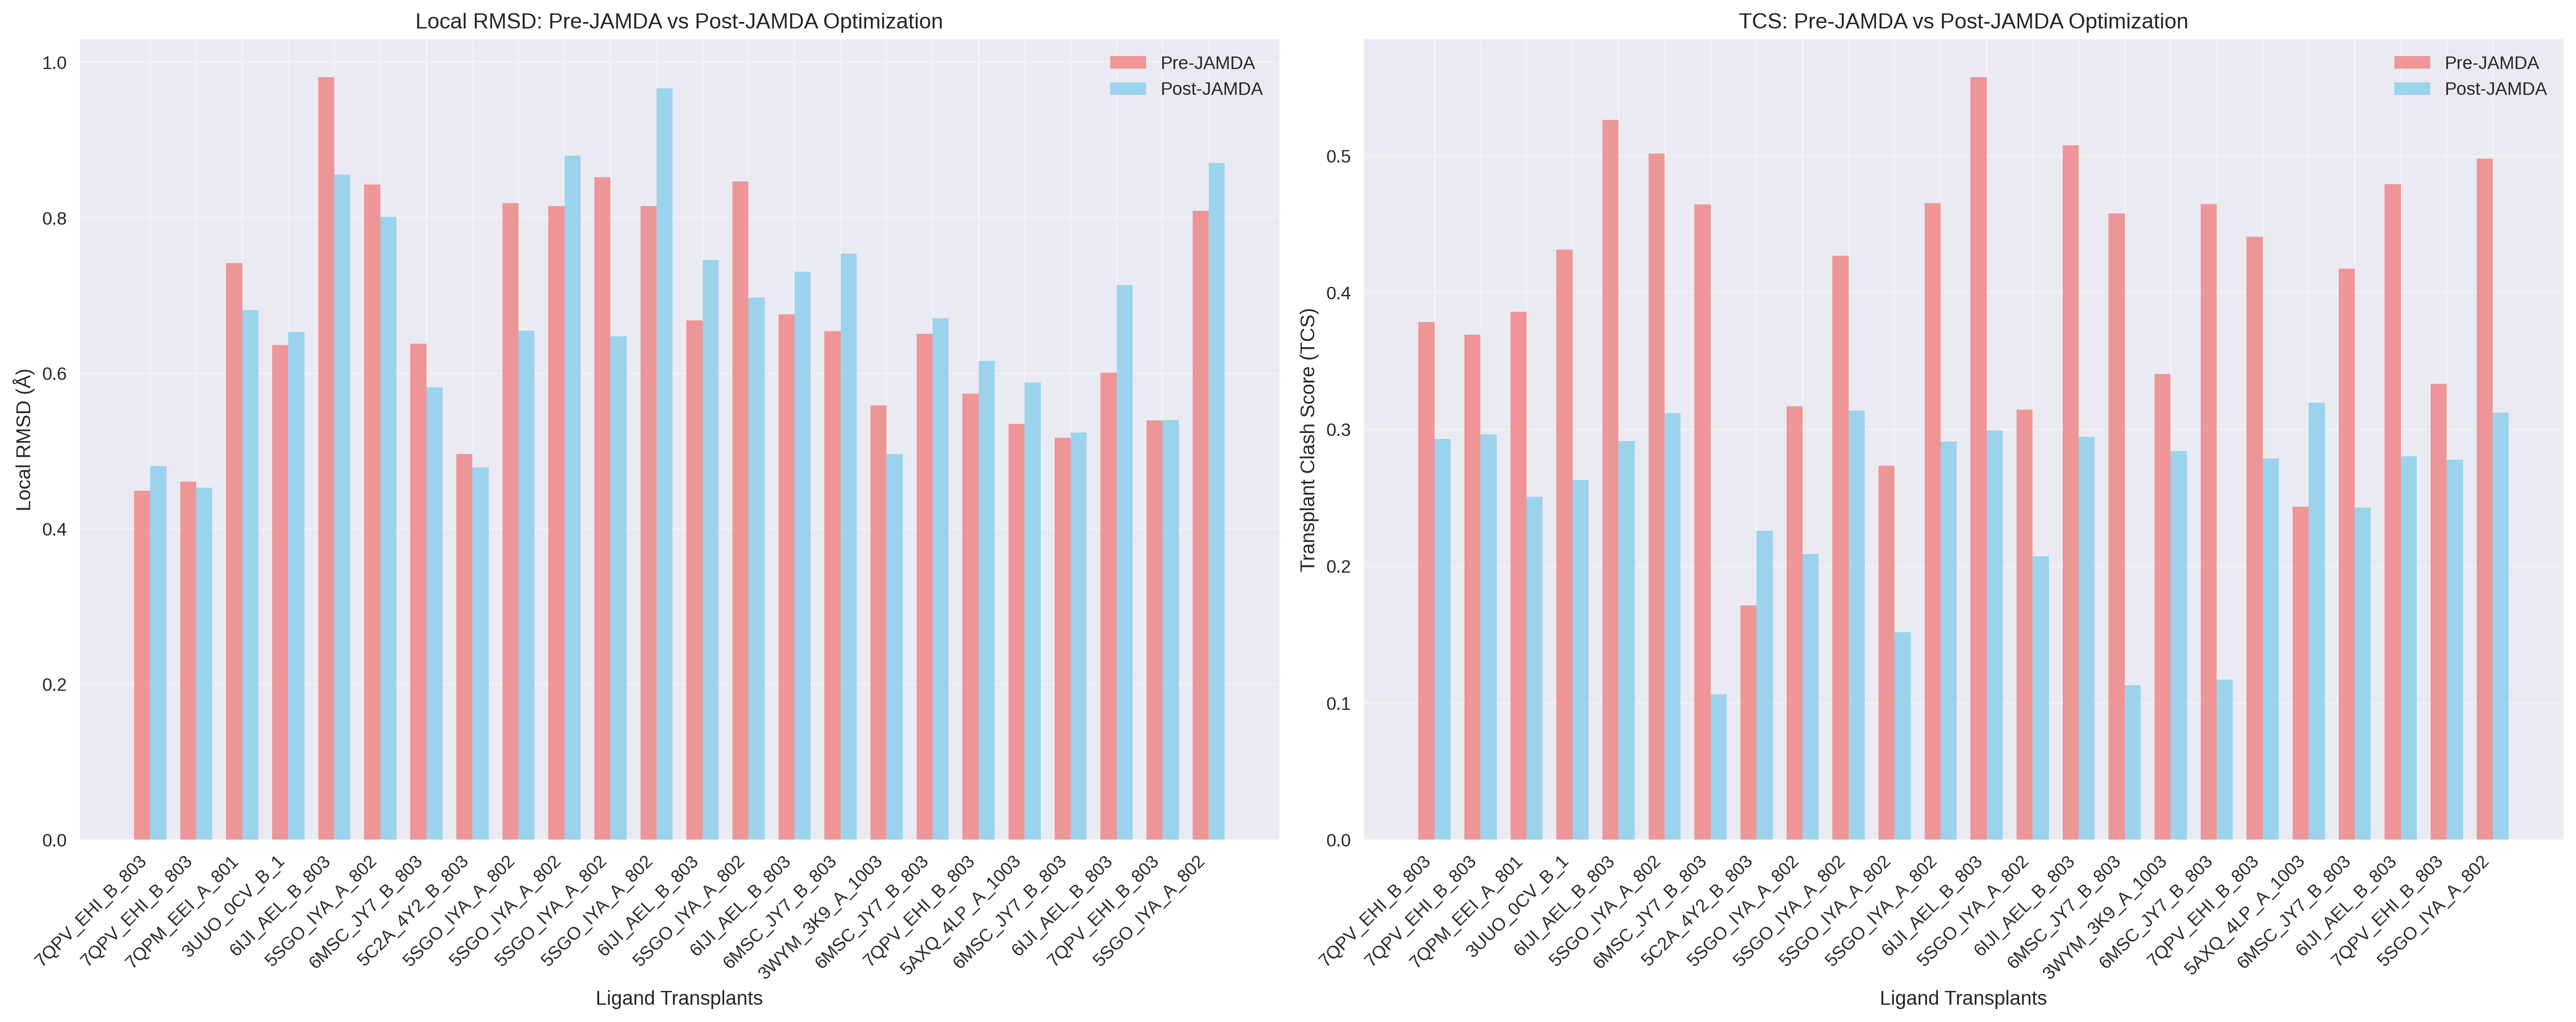
\includegraphics[width=\textwidth, keepaspectratio]{images/optimization_comparison.png}
    \end{figure}
\end{frame}
\begin{frame}{Consistent Improvements Across Diverse Transplants}
    \begin{itemize}
        \item For nearly every case, the Post-JAMDA scores are lower than the Pre-JAMDA scores.
        \item This demonstrates that the optimization procedure is robust and performs well across a wide range of different protein-ligand systems.
    \end{itemize}
\end{frame}

%---------------------------------------------------------------
\begin{frame}{Analyzing the Magnitude of Improvements}
    \begin{figure}
        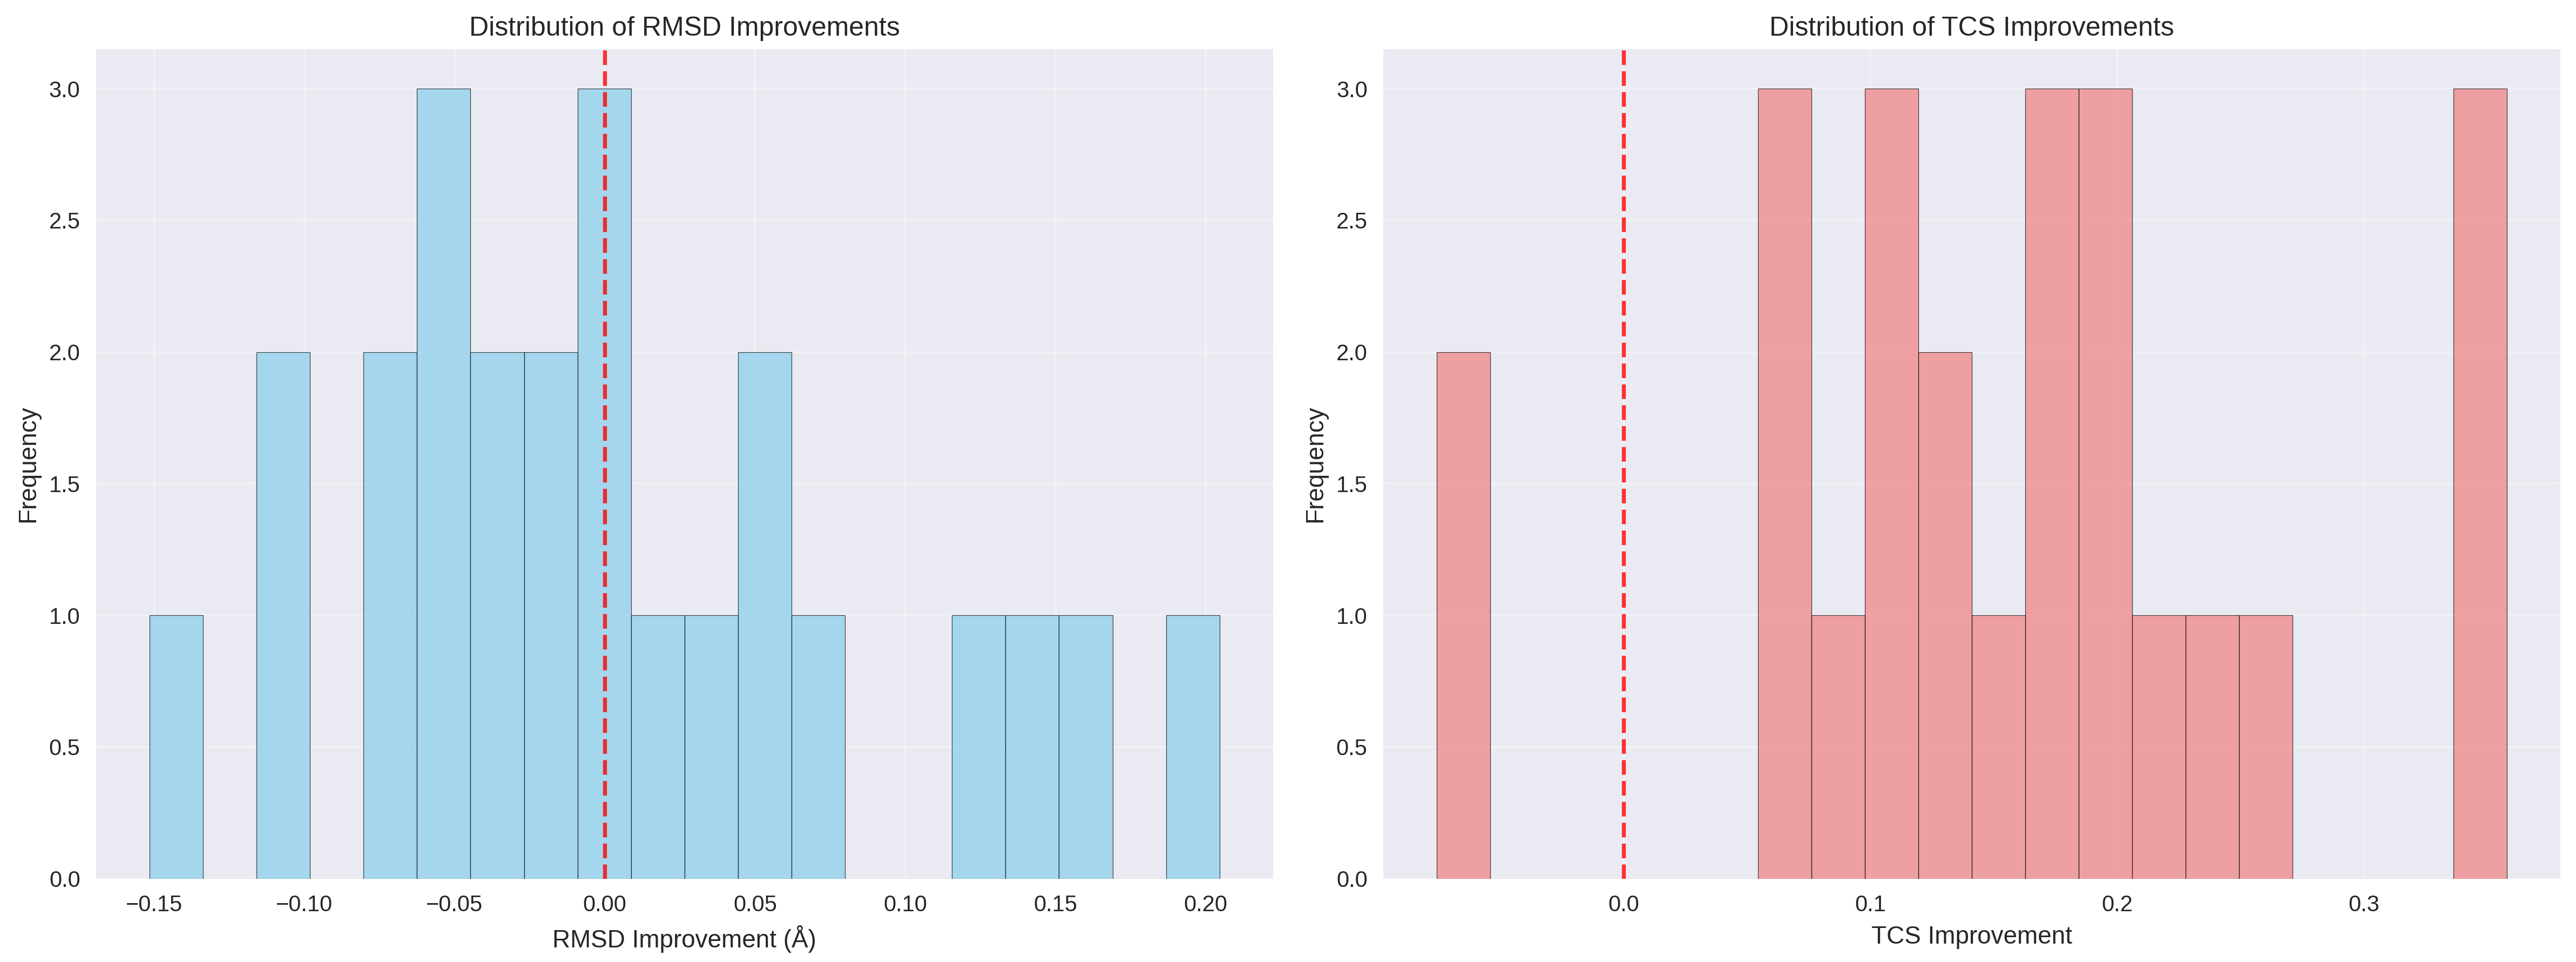
\includegraphics[width=\textwidth, keepaspectratio]{images/improvement_analysis_1.png}
    \end{figure}
\end{frame}
\begin{frame}{Analyzing the Magnitude of Improvements}
	    \begin{figure}
		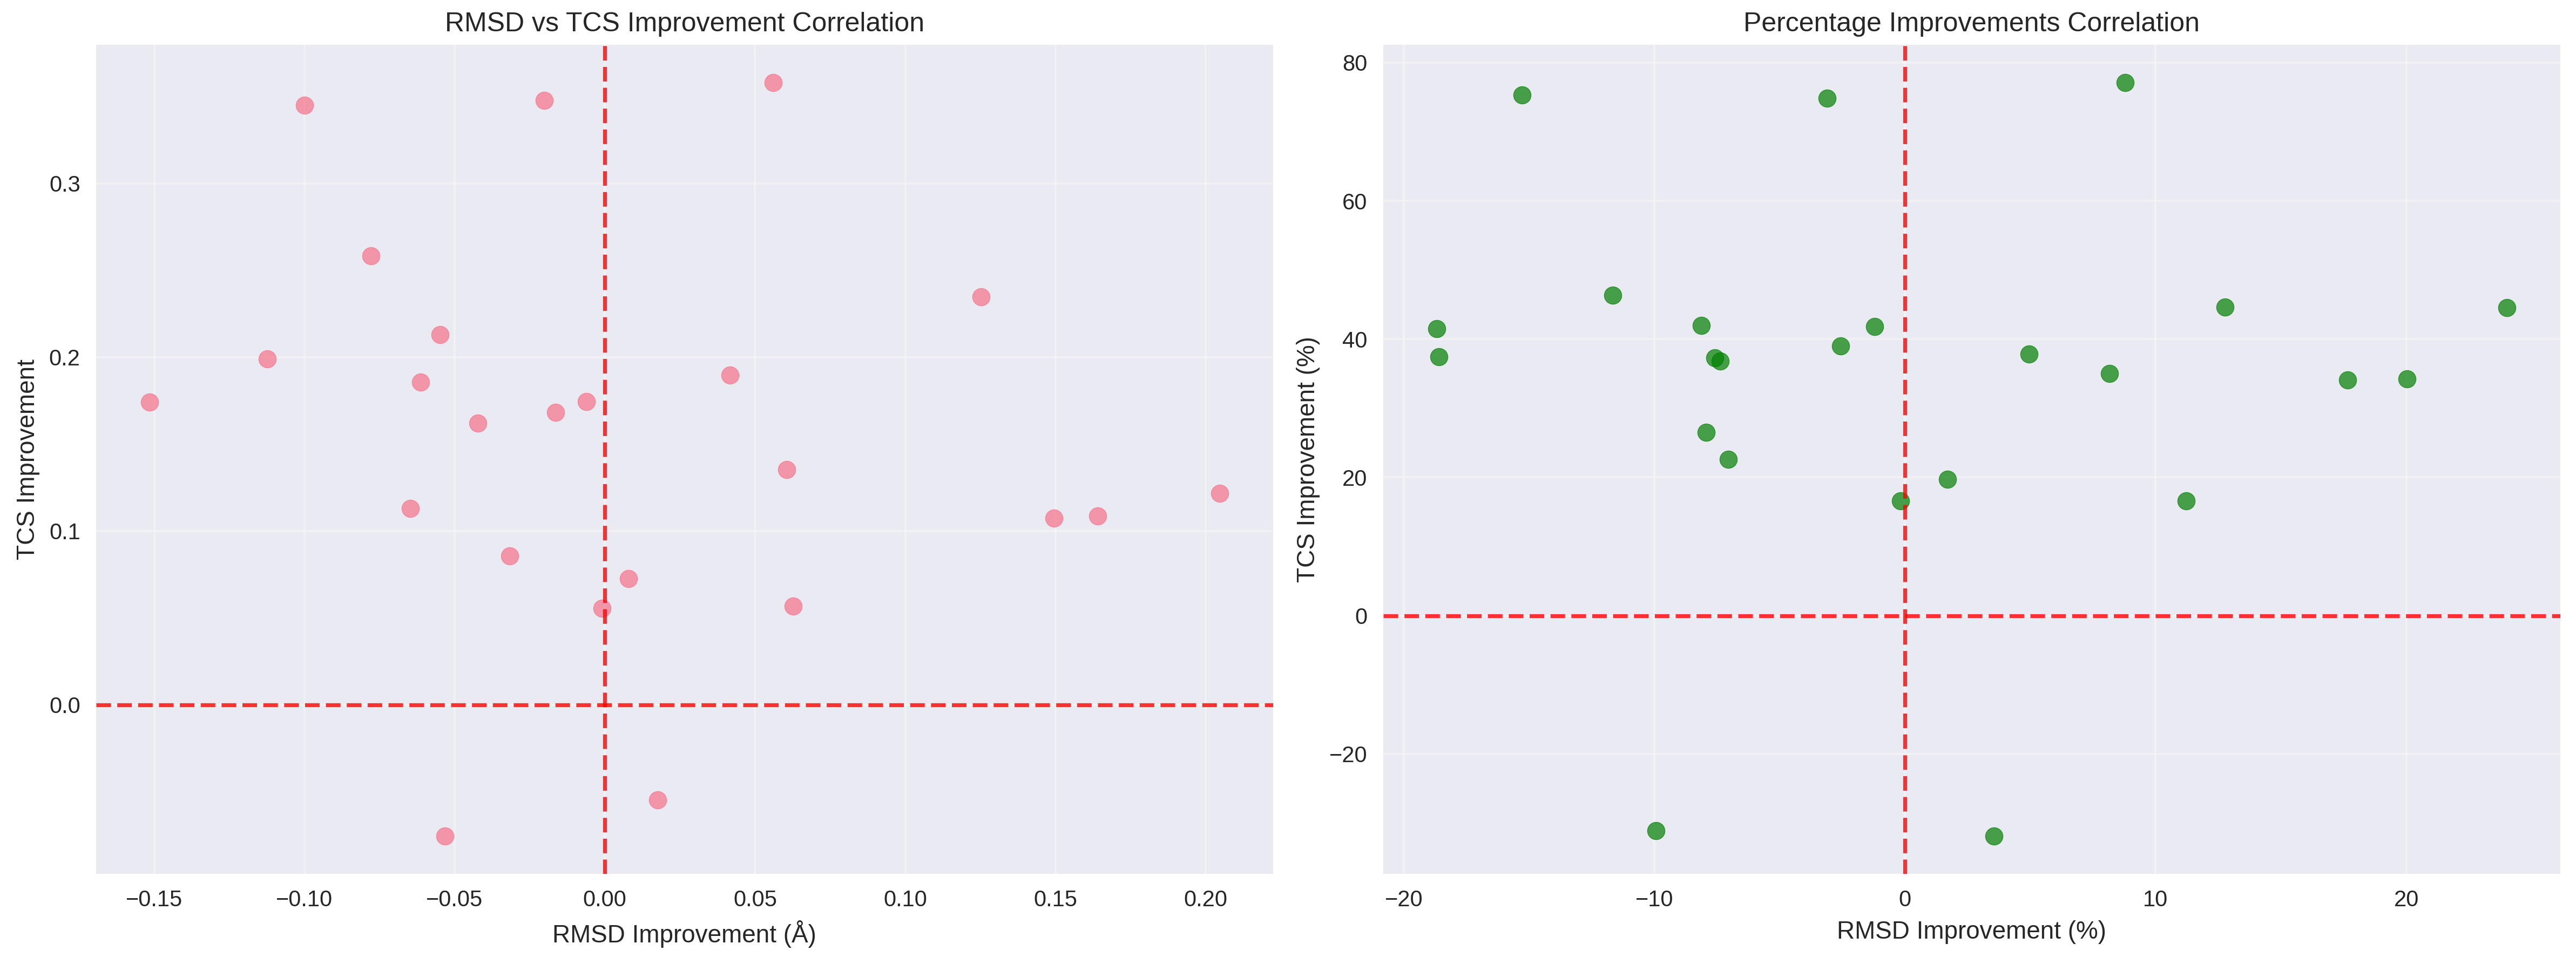
\includegraphics[width=\textwidth, keepaspectratio]{images/improvement_analysis_2.png}
	\end{figure}
\end{frame}

%---------------------------------------------------------------
\begin{frame}{Homolog Alignment Quality Moderately Correlates with Fit}
    \begin{figure}
        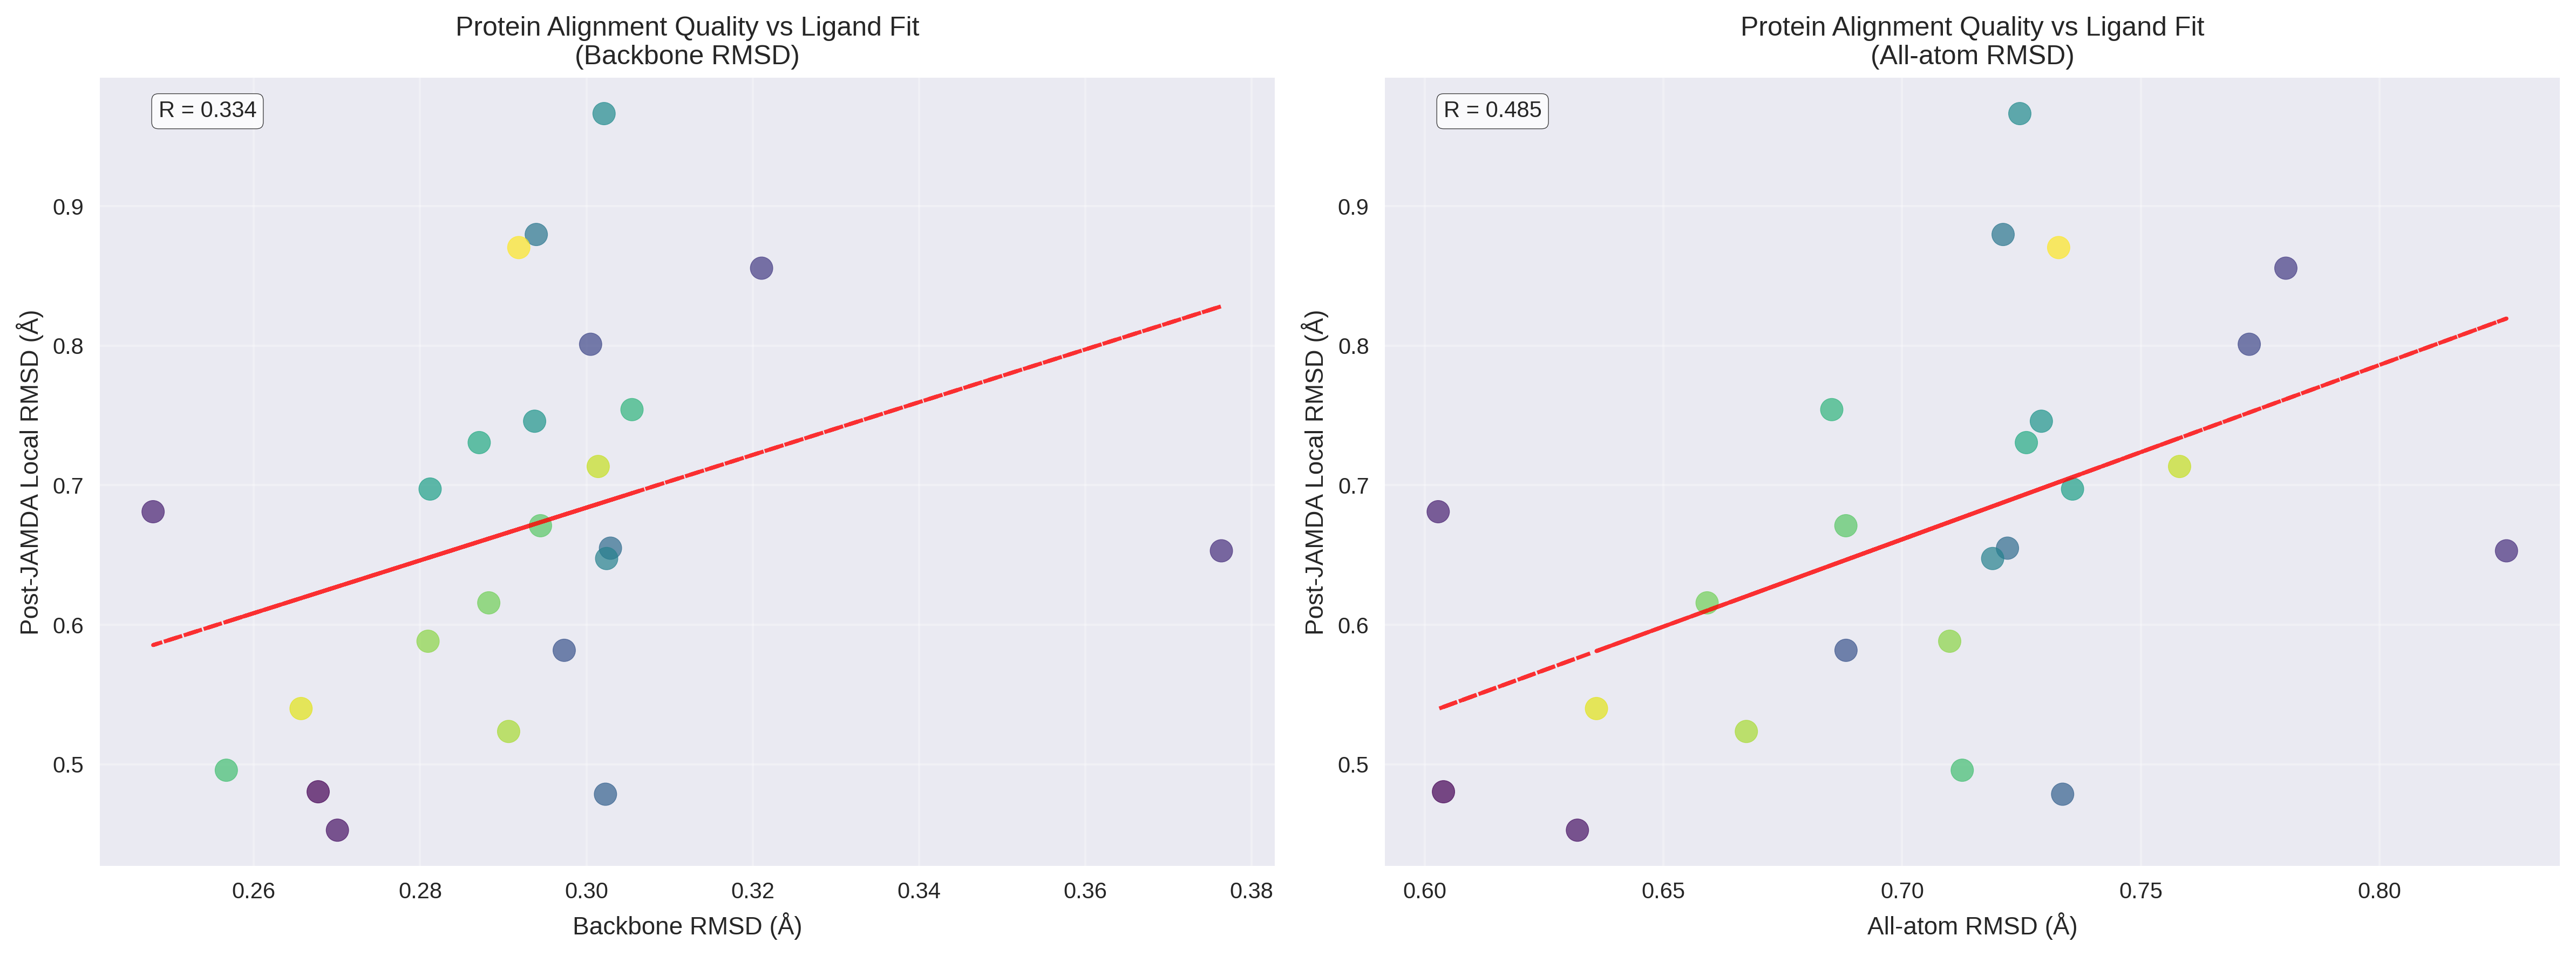
\includegraphics[width=\textwidth, keepaspectratio]{images/alignment_quality_analysis.png}
        \caption{Final ligand fit (Post-JAMDA Local RMSD) vs. the structural alignment quality of the protein.}
    \end{figure}
\end{frame}
\begin{frame}{Homolog Alignment Quality Moderately Correlates with Fit}
    \begin{itemize}
        \item We see a weak-to-moderate positive correlation ($R \approx 0.33 - 0.49$) between the initial protein alignment quality and the final ligand fit.
        \item However, the correlation is not perfect, indicating that other factors beyond simple backbone alignment are important for a successful transplant.
    \end{itemize}
\end{frame}

%---------------------------------------------------------------
\begin{frame}{Next Steps \& Roadmap}
    \begin{itemize}
        \item Benchmark Against AlphaFill
        \item Investigate Outliers
        \item Increase Dataset/ Improve Performance
        \item Develop Confidence Scores
    \end{itemize}
\end{frame}

%---------------------------------------------------------------
\begin{frame}
    \centering
    \Huge{Thank you!}
    \vfill
    \Large{Questions?}
\end{frame}

\end{document}